%% no need for  \DeclareGraphicsExtensions{.pdf,.eps}

\documentclass[12pt,letterpaper,english]{article}
\usepackage{times}
\usepackage[T1]{fontenc}
\IfFileExists{url.sty}{\usepackage{url}}
                      {\newcommand{\url}{\texttt}}

\usepackage{babel}
%\usepackage{noweb}
\usepackage{Rd}

\usepackage{Sweave}

%\VignetteIndexEntry{Performance Attribution from Bacon}
%\VignetteDepends{PerformanceAnalytics}
%\VignetteKeywords{returns, performance, risk, benchmark, portfolio}
%\VignettePackage{PerformanceAnalytics}

%\documentclass[a4paper]{article}
%\usepackage[noae]{Sweave}
%\usepackage{ucs}
%\usepackage[utf8x]{inputenc}
%\usepackage{amsmath, amsthm, latexsym}
%\usepackage[top=3cm, bottom=3cm, left=2.5cm]{geometry}
%\usepackage{graphicx}
%\usepackage{graphicx, verbatim}
%\usepackage{ucs}
%\usepackage[utf8x]{inputenc}
%\usepackage{amsmath, amsthm, latexsym}
%\usepackage{graphicx}

\title{Umsmooth Return Models Impact}
\author{Shubhankit Mohan}

\begin{document}
\Sconcordance{concordance:OWReturn.tex:OWReturn.Rnw:%
1 46 1 1 5 1 4 45 1 1 4 1 2 2 1 1 4 1 2 3 1 1 3 1 2 3 1 1 3 1 2 5 1 1 2 %
1 0 3 1 5 0 1 1 5 0 1 2 6 0 1 1 5 0 1 2 1 0 1 1 1 2 1 0 1 2 1 0 1 2 5 0 %
1 2 1 1 1 2 1 0 4 1 1 2 1 0 1 2 1 0 1 2 6 0 1 3 10 1 1 5 5 0 1 2 6 1 1 %
2 1 0 1 1 6 0 1 2 6 1 1 2 1 0 1 1 7 0 1 2 8 1 1 2 1 0 1 1 7 0 1 2 9 1 1 %
2 1 0 1 1 6 0 1 1 7 0 1 2 7 1 1 5 15 0 1 2 4 1}


\maketitle


\begin{abstract}
The fact that many hedge fund returns exhibit extraordinary levels of serial correlation is now well-known and generally accepted as fact.Because hedge fund strategies have exceptionally high autocorrelations in reported returns and this is taken as evidence of return smoothing, we first develop a method to completely eliminate any order of serial correlation across a wide array of time series processes.Once this is complete, we can determine the underlying risk factors to the "true" hedge fund returns and examine the incremental benefit attained from using nonlinear payoffs relative to the more traditional linear factors.
\end{abstract}
\tableofcontents




\section{Okunev White Model Methodology}
Given a sample of historical returns \((R_1,R_2, . . .,R_T)\),the method assumes the fund manager smooths returns in the following manner:

%Let $X \sim N(0,1)$ and $Y \sim \textrm{Exponential}(\mu)$.  Let
%$Z = \sin(X)$. $\sqrt{X}$.
  
%$\hat{\mu}$ = $\displaystyle\frac{22}{7}$
%e^{2 \mu} = 1
%\begin{equation}
%\left(\sum_{t=1}^{T} R_t/T\right) = \hat{\mu} \\
%\end{equation}
\begin{equation}
 r_{0,t}  =  \sum_{i}^{} \beta_{i}r_{0,t-i} + (1- \alpha)r_{m,t} \\
\end{equation}


\begin{equation}
where :  \sum_{i}^{} \beta_{i} = (1- \alpha) \\
\end{equation}

\(r_{0,t}\) : is the observed (reported) return at time t (with 0 adjustments' to reported returns), \\
\(r_{m,t}\) : is the true underlying (unreported) return at time t (determined by making m adjustments to reported returns). \\

The objective is to determine the true underlying return by removing the
autocorrelation structure in the original return series without making any assumptions regarding the actual time series properties of the underlying process. We are implicitly assuming by this approach that the autocorrelations that arise in reported returns are entirely due to the smoothing behavior funds engage in when reporting results. In fact, the method may be adopted to produce any desired level of autocorrelation at any lag and is not limited to simply eliminating all autocorrelations.

\section{To Remove Up to m Orders of Autocorrelation}
To remove the first m orders of autocorrelation from a given return series we would proceed in a manner very similar to that detailed in \textbf{Geltner Return}. We would initially remove the first order autocorrelation, then proceed to eliminate the second order autocorrelation through the iteration process. In general, to remove any order, m, autocorrelations from a given return series we would make the following transformation to returns:

\begin{equation}
r_{m,t}=\frac{r_{m-1,t}-c_{m}r_{m-1,t-m}}{1-c_{m}}
\end{equation}

Where  \(r_{m-1,t}\) is the series return with the first (m-1) order autocorrelation coefficient's removed.The general form for all the autocorrelations given by the process is : 
\begin{equation}
a_{m,n}=\frac{a_{m-1,n}(1+c_{m}^2)-c_{m}(1+a_{m-1,2m})}{1+c_{m}^2 -2c_{m}a_{m-1,n}}
\end{equation}

Once a solution is found for \(c_{m}\) to create \(r_{m,t}\) , one will need to iterate back to remove the first 'm'autocorrelations again. One will then need to once again remove the mth autocorrelation using the adjustment in equation (3). It would continue the process until the first m autocorrelations are sufficiently close to zero.

\section{Time Series Characteristics}

Given a series  of historical returns \((R_1,R_2, . . .,R_T)\) from \textbf{January-1997} to \textbf{January-2008}, create a wealth index chart, bars for per-period performance, and underwater chart for drawdown of the  Hedge Funds Indiciesfrom EDHEC Database.

\subsection{ Performance Summary}
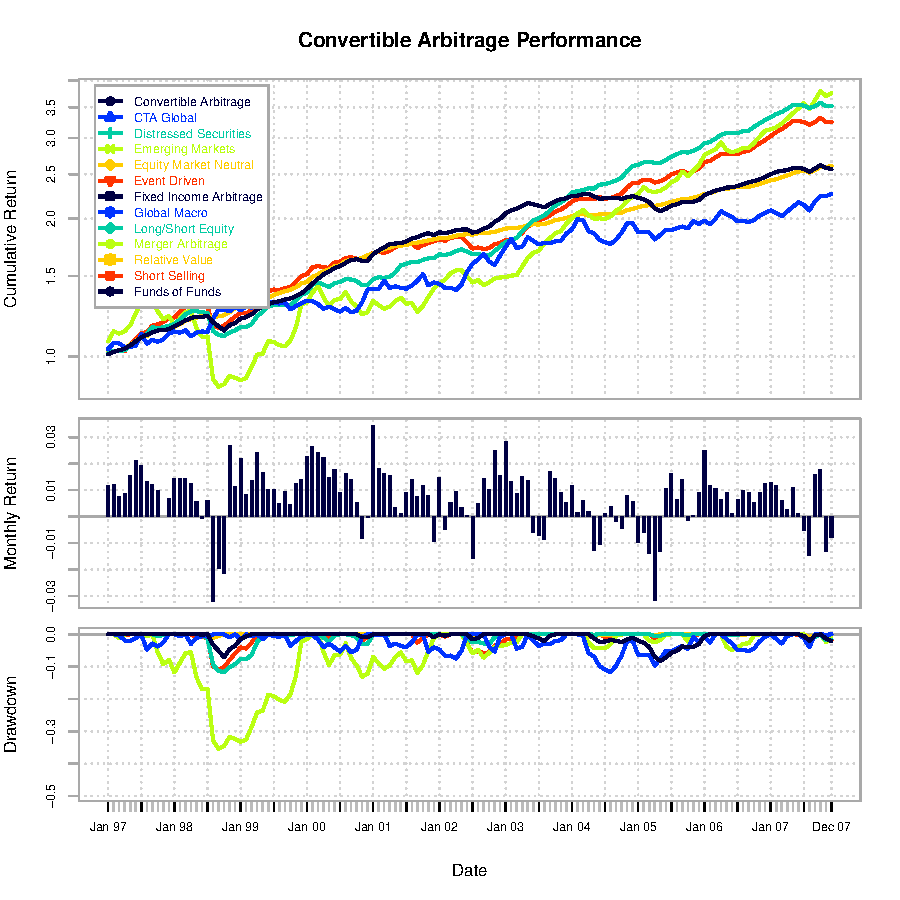
\includegraphics{OWReturn-003}

After applying the \textbf{Okunev White Model} to remove the serial correlation , we get the following Performance Chart.

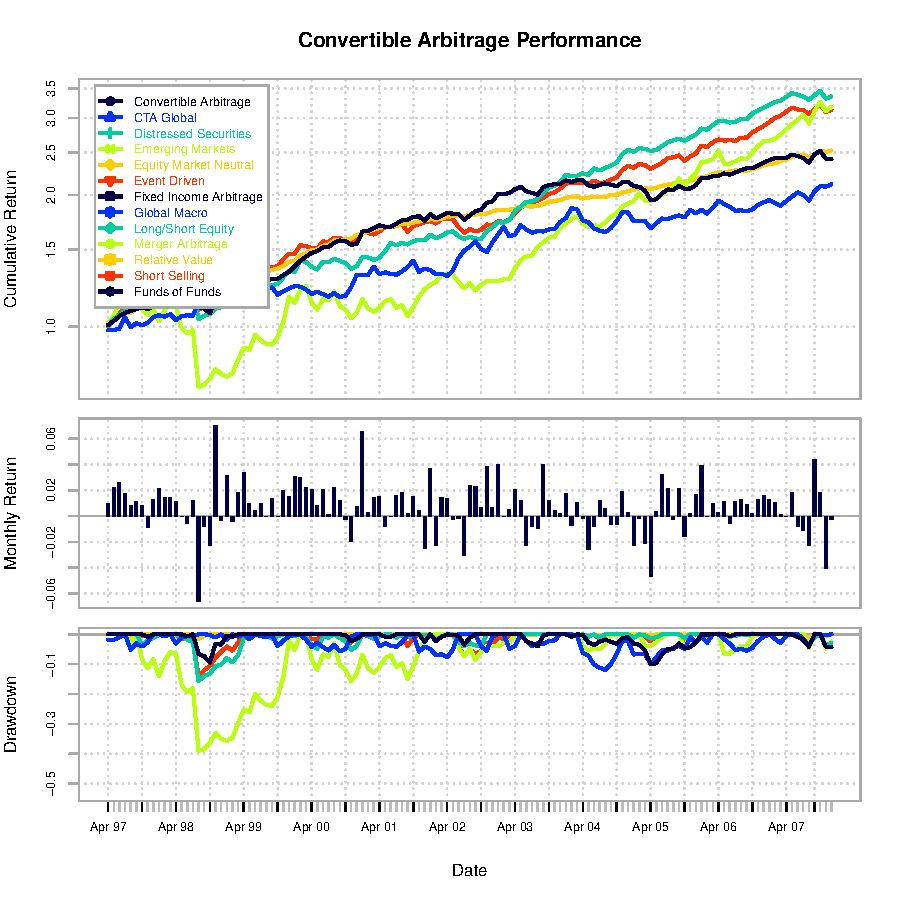
\includegraphics{OWReturn-004}

\subsection{Autocorrelation UnSmoothing Impact}
One promiment feature visible by the summary chart is the removal of \textbf{serial autocorrelation} and \textbf{unsoomthing} of the return series.The significant drop in autocorrelation, is visible by the following chart based on  indicies of the CTA global ,Distressed Securities and Ememrging Markets which had the highest autocorrelation .

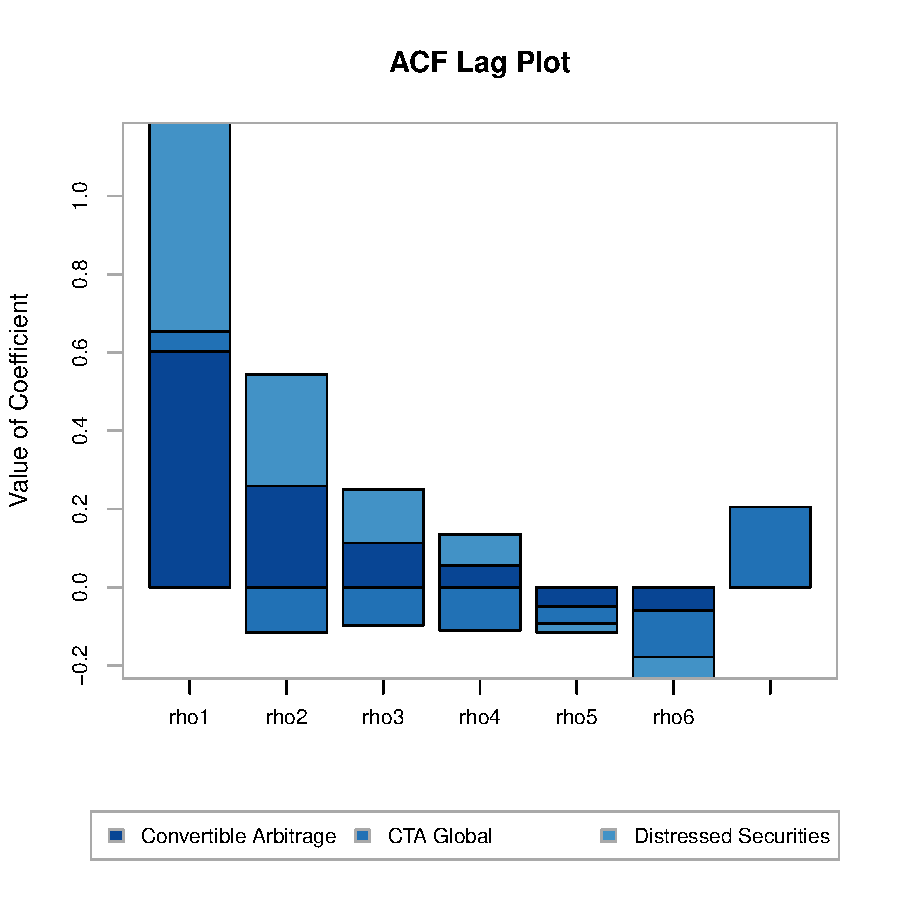
\includegraphics{OWReturn-005}

The change can be evidently seen by the following chart :


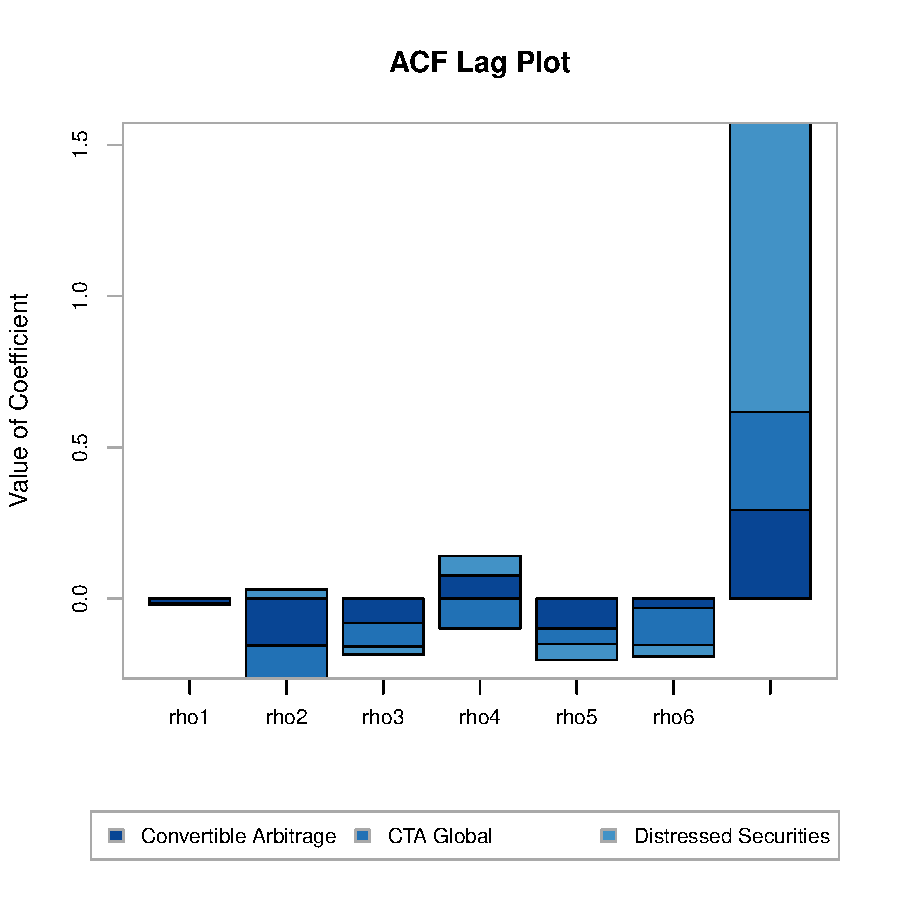
\includegraphics{OWReturn-006}


\subsection{Comparing Distributions}

In this example we use edhec database, to compute true Hedge Fund Returns.

\begin{Schunk}
\begin{Sinput}
> library(PerformanceAnalytics)
> data(edhec)
> Returns = Return.Okunev(edhec[,1])
> skewness(edhec[,1])
\end{Sinput}
\begin{Soutput}
[1] -2.683657
\end{Soutput}
\begin{Sinput}
> skewness(Returns)
\end{Sinput}
\begin{Soutput}
[1] -1.19068
\end{Soutput}
\begin{Sinput}
> # Right Shift of Returns Ditribution for a negative skewed distribution 
> kurtosis(edhec[,1])
\end{Sinput}
\begin{Soutput}
[1] 16.17819
\end{Soutput}
\begin{Sinput}
> kurtosis(Returns)
\end{Sinput}
\begin{Soutput}
[1] 10.59337
\end{Soutput}
\begin{Sinput}
> # Reduction in "peakedness" around the mean
> layout(rbind(c(1, 2), c(3, 4)))
>  chart.Histogram(Returns, main = "Plain", methods = NULL)
>  chart.Histogram(Returns, main = "Density", breaks = 40,
+  methods = c("add.density", "add.normal"))
>  chart.Histogram(Returns, main = "Skew and Kurt",
+  methods = c("add.centered", "add.rug"))
> chart.Histogram(Returns, main = "Risk Measures",
+  methods = c("add.risk"))
\end{Sinput}
\end{Schunk}
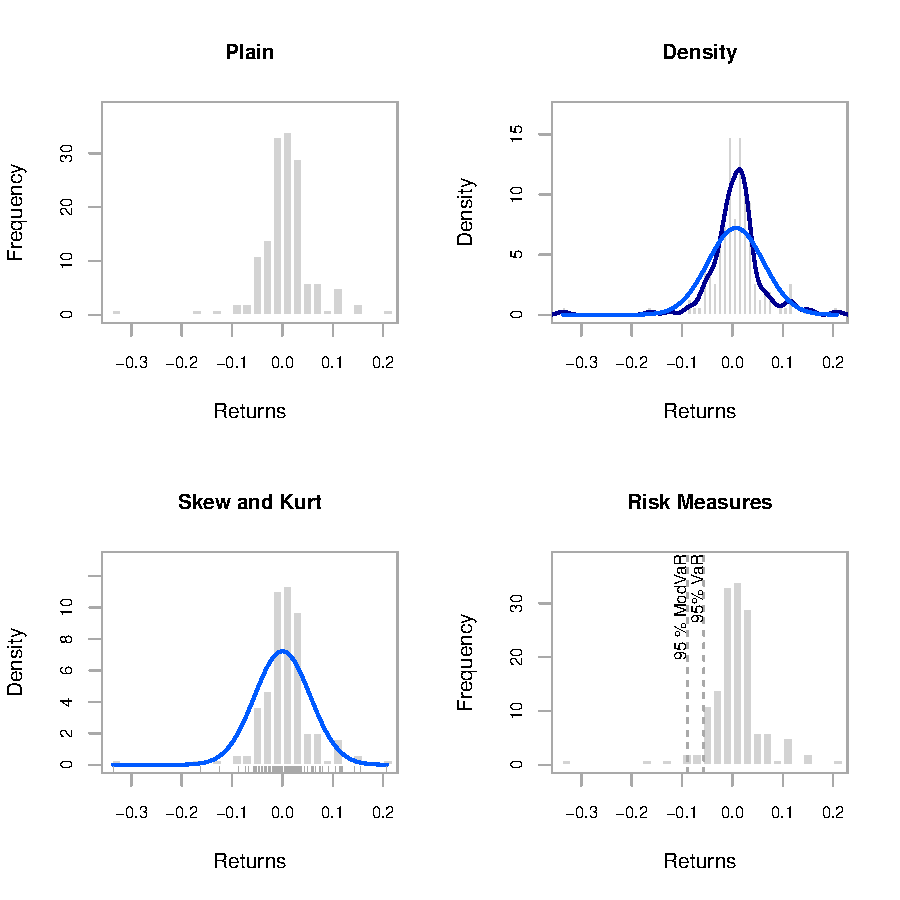
\includegraphics{OWReturn-007}

The above figure shows the behaviour of the distribution tending to a normal IID distribution.For comparitive purpose, one can observe the change in the charateristics of return as compared to the orignal.
\begin{Schunk}
\begin{Sinput}
> library(PerformanceAnalytics)
> data(edhec)
> Returns = Return.Okunev(edhec[,1])
> layout(rbind(c(1, 2), c(3, 4)))
>  chart.Histogram(edhec[,1], main = "Plain", methods = NULL)
>  chart.Histogram(edhec[,1], main = "Density", breaks = 40,
+  methods = c("add.density", "add.normal"))
>  chart.Histogram(edhec[,1], main = "Skew and Kurt",
+  methods = c("add.centered", "add.rug"))
> chart.Histogram(edhec[,1], main = "Risk Measures",
+  methods = c("add.risk"))
> 
\end{Sinput}
\end{Schunk}
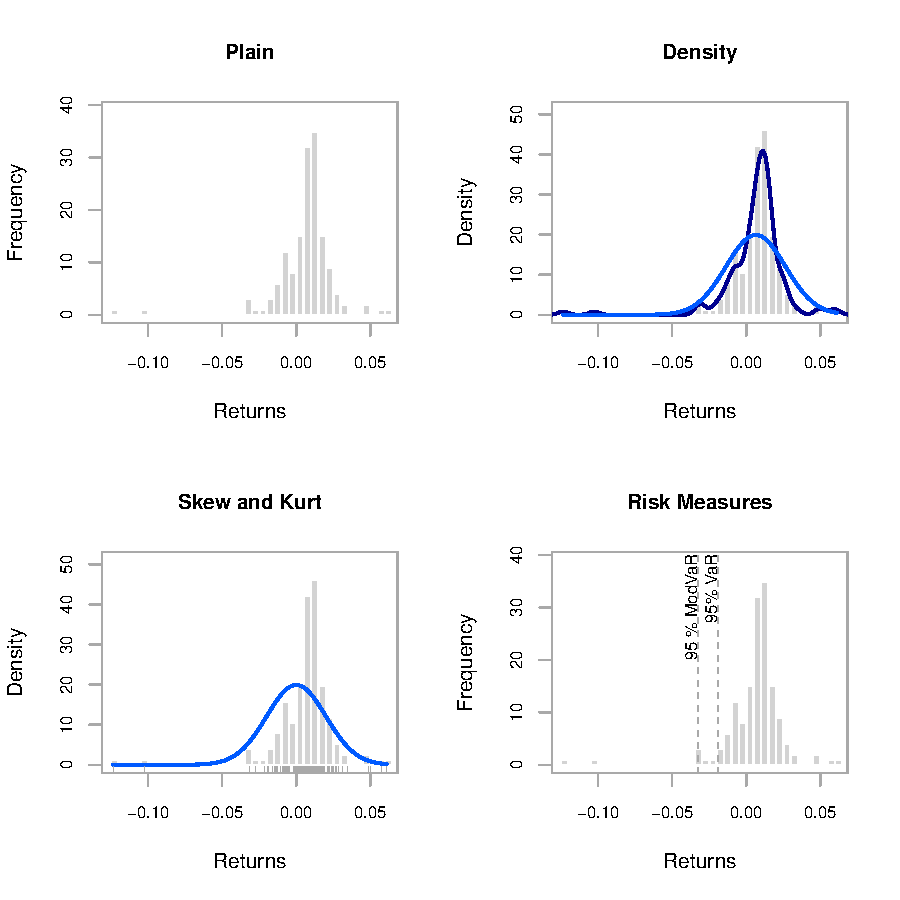
\includegraphics{OWReturn-008}

\section{Risk Measure}

\subsection{Mean absolute deviation}

To calculate Mean absolute deviation we take the sum of the absolute value of the difference between the returns and the mean of the returns and we divide it by the number of returns.

 \deqn{MeanAbsoluteDeviation = \frac{\sum^{n}_{i=1}\mid r_i - \overline{r}\mid}{n}}{MeanAbsoluteDeviation = sum(|r-mean(r)|)/n }

where \eqn{n} is the number of observations of the entire series, \eqn{r_i} is the return in month i and \eqn{\overline{r}} is the mean return

\begin{Schunk}
\begin{Soutput}
                        Convertible Arbitrage CTA Global Distressed Securities
Mean absolute deviation              191.5453   5.581807              89.59503
\end{Soutput}
\end{Schunk}

We can observe than due to the spurious serial autocorrelation, the true \textbf{volatility} was hidden, which is \textbf{more than 100 \% } in case of Distressed Securities to the one apparent to the investor.\textbf{CTA Global}, has the lowerst change, which is consistent,with the fact with it has the lowerst autocorreration.

\subsection{Frequency (p.64)}

Gives the period of the return distribution (ie 12 if monthly return, 4 if quarterly return)

\begin{Schunk}
\begin{Sinput}
> data(portfolio_bacon)
> print(Frequency(portfolio_bacon[,1])) #expected 12
\end{Sinput}
\begin{Soutput}
[1] 12
\end{Soutput}
\end{Schunk}

\subsection{Sharpe Ratio (p.64)}

The Sharpe ratio is simply the return per unit of risk (represented by variability).  In the classic case, the unit of risk is the standard deviation of the returns.
 
\deqn{\frac{\overline{(R_{a}-R_{f})}}{\sqrt{\sigma_{(R_{a}-R_{f})}}}}

\begin{Schunk}
\begin{Sinput}
> data(managers)
> SharpeRatio(managers[,1,drop=FALSE], Rf=.035/12, FUN="StdDev") 
\end{Sinput}
\begin{Soutput}
                                     HAM1
StdDev Sharpe (Rf=0.3%, p=95%): 0.3201889
\end{Soutput}
\end{Schunk}

\subsection{Risk-adjusted return: MSquared (p.67)}

\eqn{M^2} is a risk adjusted return useful to judge the size of relative performance between differents portfolios. With it you can compare portfolios with different levels of risk.

\deqn{M^2 = r_P + SR * (\sigma_M - \sigma_P) = (r_P - r_F) * \frac{\sigma_M}{\sigma_P} + r_F}{M squared = Rp + SR * (Market risk - Portfolio risk) = (Rp - Rf) * Market risk / Portfolio risk + Rf}

where \eqn{r_P}. is the portfolio return annualized, \eqn{\sigma_M}. is the market risk and \eqn{\sigma_P} is the portfolio risk

\begin{Schunk}
\begin{Sinput}
> data(portfolio_bacon)
> print(MSquared(portfolio_bacon[,1], portfolio_bacon[,2])) #expected 0.1068
\end{Sinput}
\begin{Soutput}
                             portfolio.monthly.return....
portfolio.monthly.return....                    0.1068296
\end{Soutput}
\end{Schunk}

\subsection{MSquared Excess (p.68)}

\eqn{M^2} excess is the quantity above the standard M. There is a geometric excess return which is better for Bacon and an arithmetic excess return

\deqn{M^2 excess (geometric) = \frac{1 + M^2}{1 + b} - 1}{MSquared excess (geometric) = (1+M^2)/(1+b) - 1}
\deqn{M^2 excess (arithmetic) = M^2 - b}{MSquared excess (arithmetic) = M^2 - b}

where \eqn{M^2}. is MSquared and \eqn{b}. is the benchmark annualised return.

\begin{Schunk}
\begin{Sinput}
> data(portfolio_bacon)
> print(MSquaredExcess(portfolio_bacon[,1], portfolio_bacon[,2])) #expected -0.00998
\end{Sinput}
\begin{Soutput}
                             portfolio.monthly.return....
portfolio.monthly.return....                 -0.009976721
\end{Soutput}
\begin{Sinput}
> print(MSquaredExcess(portfolio_bacon[,1], portfolio_bacon[,2], Method="arithmetic")) #expected -0.011
\end{Sinput}
\begin{Soutput}
                             portfolio.monthly.return....
portfolio.monthly.return....                  -0.01115381
\end{Soutput}
\end{Schunk}


\section{Downside Risk}
As we have obtained the true hedge fund returns, what is the actual \textbf{VaR,drawdown and downside potential} of the indices, can be illustrated by the following example, where we CTA Global and Distressed Securities indicies have been as sample sata sets.

The following table, shows the change in \textbf{absolute value} in terms of percentage, when the Okunev White Return model has been implemented as compared to the Orginal model. We can observe, that for the given period , before the 2008 financial crisis, the hedge fund returns have a \textbf{100} \% increase in exposure.The result is consistent , when tested on other indicies, which show that true risk was camouflaged under the haze of smoothing in the hedge fund industry.


\begin{Schunk}
\begin{Soutput}
                             CTA Global Distressed Securities
Semi Deviation                 5.780347              75.67568
Gain Deviation                 1.775148              70.19231
Loss Deviation                 7.407407              48.18653
Downside Deviation (MAR=10%)   6.521739              75.16779
Downside Deviation (Rf=0%)     8.759124              89.07563
Downside Deviation (0%)        8.759124              89.07563
Maximum Drawdown               2.568493              17.88831
Historical VaR (95%)           5.932203              86.24339
Historical ES (95%)            5.518764              77.75176
Modified VaR (95%)             7.988166              96.72727
Modified ES (95%)              8.644860              85.38588
\end{Soutput}
\end{Schunk}

\section{Impact on Performance Ratios}


\end{document}
